% \section*{Part 1}

% Using the instructions provided in the project description, run memcached alone (i.e., no interference), and with each iBench source of interference (cpu, l1d, l1i, l2, llc, membw). For Part 1, you must use the following \texttt{mcperf} command, which varies the target QPS from 5000 to 80000 in increments of 5000 (and has a warm-up time of 2 seconds with the addition of \texttt{-w 2}):

% \begin{verbatim}
% $ ./mcperf -s MEMCACHED_IP --loadonly
% $ ./mcperf -s MEMCACHED_IP -a INTERNAL_AGENT_IP  \
%            --noload -T 8 -C 8 -D 4 -Q 1000 -c 8 -w 2 -t 5 \ 
%            --scan 5000:80000:5000
% \end{verbatim}

% \noindent Repeat the run for each of the 7 configurations (without interference, and the 6 interference types) {\color{red} \textbf{at least 3 times}} (3 should be sufficient in this case), and collect the performance measurements (i.e. the \texttt{client-measure} VM output).

% \noindent\textbf{\underline{Reminder:}} after you have collected all the measurements, make sure you \textbf{{\color{red}delete your cluster}}. Otherwise, you will easily use up the cloud credits. See the project description for instructions how to make sure your cluster is deleted.

% %%%%%%%%%%%%%%%%%%%%%%%%%%%%%%%%%%%%%%%%%%%
% %%% QUESTION 1A

% \begin{enumerate}[label=(\alph*)]
%     \setcounter{enumi}{0}

%     \item Plot a line graph with the following stipulations:
%     \begin{itemize}
%         \item Queries per second (QPS) on the x-axis (the x-axis should range from 0 to 80K).\\
%         (\textbf{note:} the actual achieved QPS, not the target QPS)
%         \item 95th percentile latency on the y-axis (the y-axis should range from 0 to 6 ms).%la nostra è 0-14?
%         \item Label your axes.
%         \item 7 lines, one for each configuration. Add a legend.
%         \item State how many runs you averaged across and include error bars at each point in both dimensions.
%         % \item The readability of your plot will be part of your grade.
%     \end{itemize}
    
%     % \textbf{The shape of the curves depends on many factors and may differ across groups. However, that does not imply that your solutions are wrong.} 
    
% \end{enumerate}

% \textbf{Answer:}

% \begin{figure}[H]
%     \centering
%     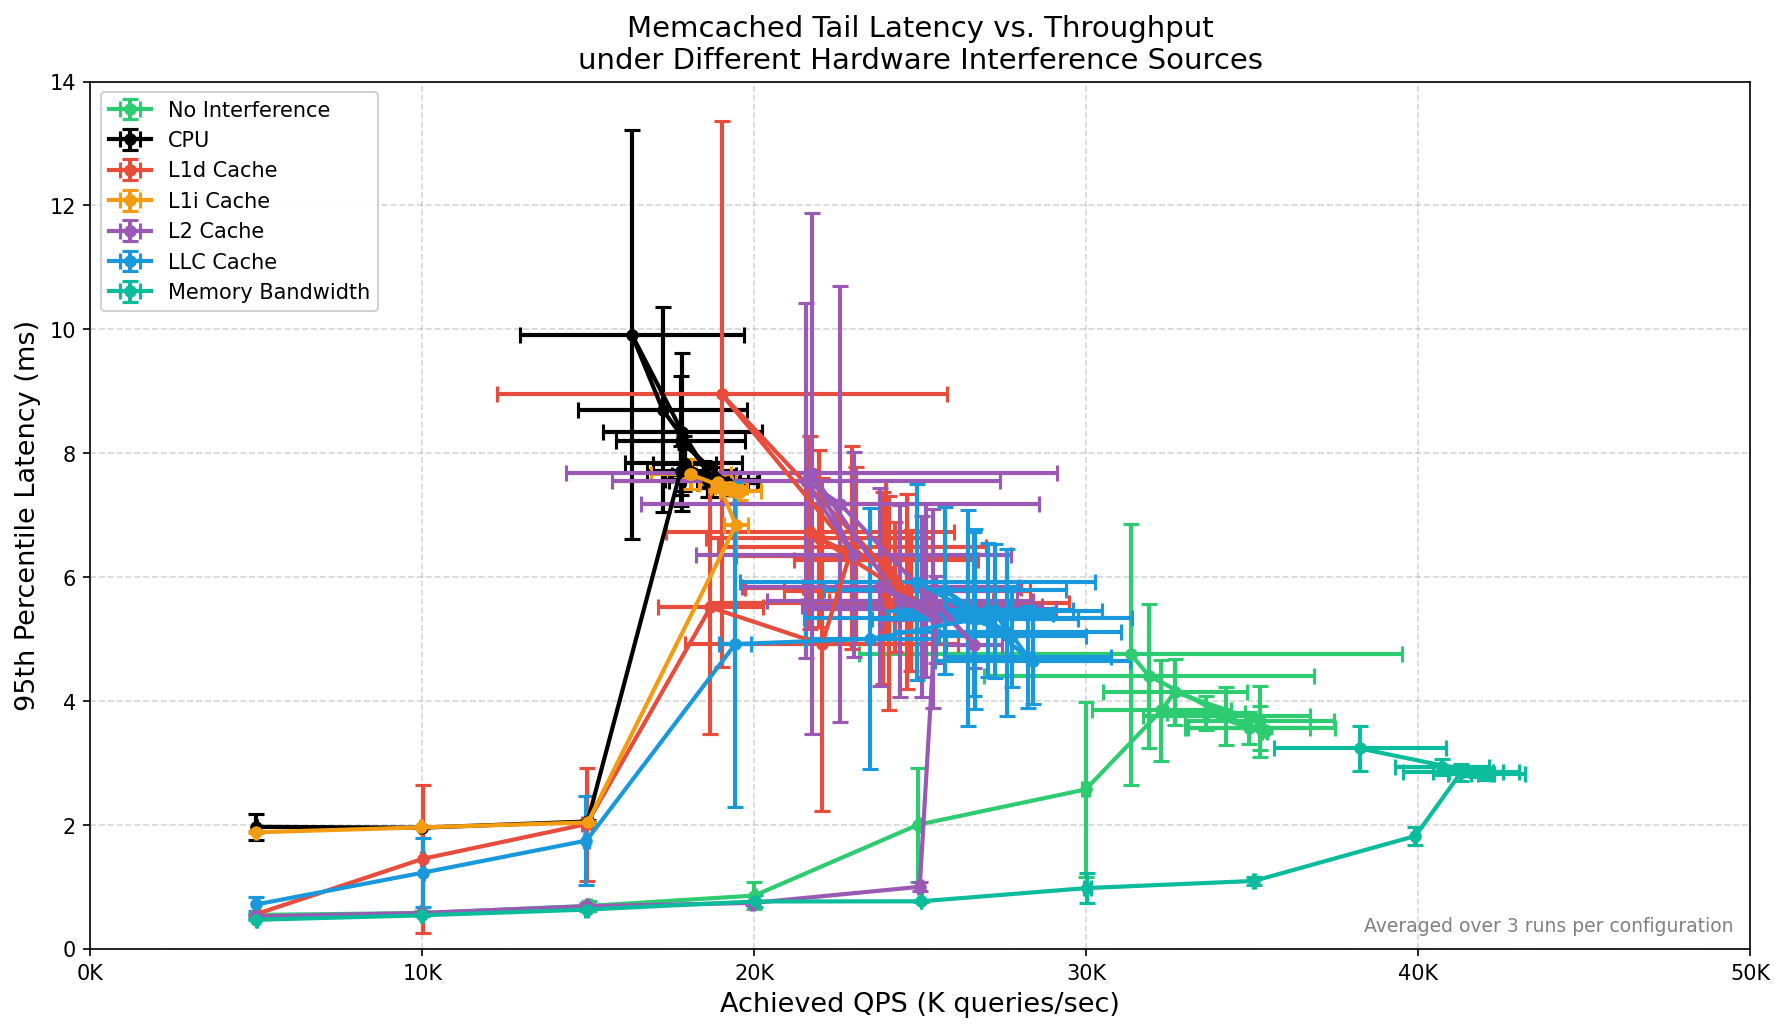
\includegraphics[width=0.70\linewidth]{Project Template/figures/part1_latency_plot.png}
%     \caption{Latency Plot}
%     \label{fig:placeholder}
% \end{figure}
% %%%%%%%%%%%%%%%%%%%%%%%%%%%%%%%%%%%%%%%%%%%
% %%% QUESTION 1B
% \newpage
% \begin{enumerate}[label=(\alph*)]
%     \setcounter{enumi}{1}
    
%     \item How is the tail latency and saturation point (the “knee in the curve”) of memcached affected by each type of interference? What is your reasoning for these effects? Briefly describe your hypothesis.
    
% \end{enumerate}

% \textbf{Answer:}
% \begin{itemize}
%     \item \texttt{ibench-cpu}: Strongest interference. Saturation knee shifts left to
%     $\sim$15--17K QPS, with tail latency reaching $\sim$8--10\,ms and high variance
%     across runs.

%     \textit{Explanation:} ibench-cpu competes directly with memcached for CPU cycles.
%     The OS scheduler time-multiplexes the cores between the two processes, leaving
%     memcached with significantly less execution time. Each incoming request must wait
%     longer to be processed, causing the server to saturate at a much lower throughput.
%     The high variance is explained by non-deterministic scheduling decisions.

%     \item \texttt{ibench-l1d}: Saturation knee at $\sim$17--20K QPS, tail latency
%     $\sim$7--8\,ms, with notably high variance across runs.

%     \textit{Explanation:} ibench-l1d continuously evicts cache lines from the L1 data
%     cache by performing frequent loads and stores to distinct memory locations.
%     Memcached is data-intensive: it performs hashtable lookups and accesses key-value
%     pairs on every request. When this data is evicted from L1d, memcached incurs
%     cache misses and must fetch data from L2 or deeper, adding latency per request.
%     The high variance reflects that the impact depends on which keys are requested and
%     whether their data happens to still reside in L1d or not.

%     \item \texttt{ibench-l1i}: Saturation knee at $\sim$17--19K QPS, tail latency
%     $\sim$7--8\,ms, behaving very similarly to ibench-cpu.

%     \textit{Explanation:} Memcached has very tight, frequently executed hot paths
%     (request parsing, hashtable lookup, response serialization). These instruction
%     sequences naturally reside in L1i. ibench-l1i continuously loads new instructions,
%     evicting memcached's hot code from the instruction cache. Every request then incurs
%     instruction cache misses, stalling the pipeline while instructions are re-fetched
%     from L2. This penalty effectively mimics CPU cycle theft, explaining the similarity
%     with ibench-cpu in the plot.
%      %%forse un pelo ambigua
%     \item \texttt{ibench-l2}: Moderate impact. Saturation knee at $\sim$25--28K QPS,
%     tail latency $\sim$5--7\,ms.

%     \textit{Explanation:} L2 cache is larger than L1 ($\sim$256\,KB--1\,MB per core),
%     so ibench-l2 must generate much higher memory pressure to cause significant
%     evictions of memcached's working set. Memcached can still keep its most critical
%     data in L1, partially shielding itself. When an L2 miss does occur, the penalty
%     is higher (data must be fetched from LLC), but this happens less frequently than
%     with L1 interference, resulting in a milder overall effect.

%     \item \texttt{ibench-llc}: Moderate-to-mild impact. Saturation knee at
%     $\sim$28--32K QPS, tail latency $\sim$5--6\,ms.

%     \textit{Explanation:} The LLC is large ($\sim$15--30\,MB) and shared across all
%     cores. ibench-llc must therefore generate enormous memory traffic to meaningfully
%     displace memcached's working set. For low-to-moderate QPS, most of memcached's
%     hot data still fits in LLC. When eviction does occur, the penalty is severe
%     (DRAM access, $\sim$100 cycles), explaining the moderately elevated tail latency
%     at saturation. The effect is less pronounced than L1/L2 interference because the
%     LLC's size provides a larger buffer.

%     \item \texttt{ibench-membw}: Least impactful. Saturation knee at $\sim$40K QPS,
%     tail latency $\sim$3\,ms, close to the no-interference baseline.

%     \textit{Explanation:} ibench-membw saturates the DRAM memory bus without
%     evicting cache contents. Since memcached's working set (keys, values, hashtable)
%     fits largely within the LLC, most requests are served from cache and do not require
%     DRAM accesses. Therefore, saturating memory bandwidth has minimal effect on
%     memcached's performance. This observation supports the conclusion that
%     \textbf{memcached is cache-bound, not memory-bandwidth-bound}.
% \end{itemize}

% %%%%%%%%%%%%%%%%%%%%%%%%%%%%%%%%%%%%%%%%%%%
% %%% QUESTION 1C

% \begin{enumerate}[label=(\alph*)]
%     \setcounter{enumi}{2}
%     \item Processor affinity:
%     \begin{itemize}
%         \item Explain the use of the \texttt{taskset} command in the container commands for memcached and iBench in the provided scripts.
        
%         \textbf{Answer:} % Here you place your solution.
%         The \texttt{taskset} command pins a process to a specific CPU core (or set of
%         cores) using a CPU affinity mask. In the provided scripts, \texttt{taskset} is
%         used to bind the memcached server to a fixed core (e.g., core~0) and to place
%         each iBench benchmark on either the \emph{same} core as memcached or a
%         \emph{different} core, depending on which hardware resource is being stressed.
%         This ensures that the interference is controlled and reproducible: without
%         \texttt{taskset}, the OS scheduler could freely migrate processes across cores,
%         making it impossible to target a specific shared resource and producing
%         inconsistent results across runs.

%         \item Why do we run some of the iBench benchmarks on the same core as memcached and others on a different core? Give an explanation for each iBench benchmark.

%         \textbf{Answer:} 
%         The choice of same vs.\ different core depends on whether the resource being
%         stressed is \emph{per-core private} or \emph{shared across cores}:

%         \begin{itemize}
%             \item \texttt{ibench-cpu}: run on the \textbf{same core} as memcached.
%             CPU cycles are a per-core resource. To actually steal execution time from
%             memcached, ibench must compete on the exact same core; running on a
%             different core would have no effect on memcached's available CPU time.

%             \item \texttt{ibench-l1d}: run on the \textbf{same core} as memcached.
%             The L1d cache is private to each core. Only a process running on the same
%             core shares the same L1d, so ibench must be co-located to evict
%             memcached's data from it.

%             \item \texttt{ibench-l1i}: run on the \textbf{same core} as memcached.
%             Same reasoning as L1d — the L1 instruction cache is per-core private.
%             ibench must run on the same core to pollute memcached's instruction
%             working set.

%             \item \texttt{ibench-l2}: run on the \textbf{same core} as memcached.
%             The L2 cache is also a per-core private resource. Co-location is required
%             to cause cache evictions that affect memcached's L2 working set.

%             \item \texttt{ibench-llc}: run on a \textbf{different core} from
%             memcached. The LLC (Last Level Cache) is \emph{shared} across all cores.
%             ibench can therefore pollute the shared LLC from any core, and there is no
%             need to co-locate. Running it on a separate core also avoids conflating
%             LLC interference with CPU cycle contention.

%             \item \texttt{ibench-membw}: run on a \textbf{different core} from
%             memcached. The memory bus and DRAM bandwidth are system-wide shared
%             resources. ibench-membw saturates the memory controller and DRAM channels
%             from any core; it does not need to share a core with memcached to produce
%             its effect.
%              \end{itemize}
%     \end{itemize}
    
% \end{enumerate}

% %%%%%%%%%%%%%%%%%%%%%%%%%%%%%%%%%%%%%%%%%%%
% %%% QUESTION 1D
    
% \begin{enumerate}[label=(\alph*)]
%     \setcounter{enumi}{3}
    
%     \item Assuming a service level objective (SLO) for memcached of up to 2~ms 95th percentile latency at 35K QPS, which iBench source of interference can safely be collocated with memcached without violating this SLO? Briefly explain your reasoning.
            
% \end{enumerate}

% \textbf{Answer:}
% Only \texttt{ibench-membw} can be safely co-located with memcached without violating the SLO of $\leq$2\,ms p95 latency at 35K~QPS.
% From the plot, at an achieved throughput of 35K~QPS, all interference sources except \texttt{ibench-membw} push the 95th percentile latency well above 2\,ms (ranging from $\sim$5\,ms for LLC and L2 up to $\sim$8--10\,ms for CPU and L1
% caches). \texttt{ibench-membw} is the only configuration that keeps tail latency at approximately 1.0 \,ms at 35K~QPS, just within the SLO budget.
% The reasoning follows directly from the analysis in part~(b): memcached's working set fits largely in the LLC, so it rarely accesses DRAM. Saturating memory bandwidth therefore has negligible impact on memcached's service rate and tail latency. All other interference sources target resources that memcached actively relies on (CPU cycles, L1/L2/LLC cache capacity), causing its saturation point to
% shift well below 35K~QPS and its tail latency to far exceed the 2\,ms threshold.

% %%%%%%%%%%%%%%%%%%%%%%%%%%%%%%%%%%%%%%%%%%%
% %%% QUESTION 1E
    
% \begin{enumerate}[label=(\alph*)]
%     \setcounter{enumi}{4}
    
%     \item In the lectures you have seen queueing theory. 
%     \begin{itemize}
%         \item Is the project experiment above (ignoring client measure) an open system or a closed system? Explain why.

%         \textbf{Answer:} % Here you place your solution.
%         The experiment is a closed system. In a closed system, the number of clients (sources of requests) is fixed and finite: a client sends a request, waits for the response, and only then can issue the next request. In the mcperf setup, the client-agent and client-measure machines run a fixed number of connections (-C 8 connections per thread, -T 8 threads), each of which follows the think-time/response cycle. There is no external, unbounded arrival process; the total number of requests in flight is bounded by the number of active connections.



%         \item What is the number of clients in the system? How did you find this number?

%         \textbf{Answer:} 

%         The number of clients is $N = T \times C = 8 \times 8 = \mathbf{64}$,
%         where $T$ is the number of mcperf threads (\texttt{-T 8}) and
%         $C$ is the number of TCP connections per thread (\texttt{-C 8}).
%         Each connection corresponds to one client that keeps exactly one
%         request outstanding at all times.
%         This value can be read directly from the mcperf command used
%         during measurement:
%         \begin{verbatim}
%         ./mcperf -s <IP> -a <AGENT_IP> --noload \
%                  -T 8 -C 8 -D 4 -Q 1000 -c 8 -t 360 ...
%         \end{verbatim}

%         \item Sketch a diagram of the queueing system modeling the experiment above. Give a brief explanation of the sketch.
   
%         \textbf{Answer:} \begin{center}
% \begin{tikzpicture}[
%     box/.style={draw, minimum width=1.4cm, minimum height=0.8cm, align=center},
%     arr/.style={->, thick}
% ]
% % Clients pool
% \node[draw, rounded corners, minimum width=1.8cm, minimum height=1.2cm,
%       align=center] (clients) at (0,0) {$N=64$\\clients};

% % Think box (Z=0)
% \node[box] (think) at (3,0) {Think\\$Z=0$};

% % Queue
% \node[box, minimum width=0.7cm] (queue) at (6.2,0) {Queue};

% % Server
% \node[box] (server) at (8.5,0) {Server\\$\mu$};

% % Arrows
% \draw[arr] (clients) -- node[above]{\small dispatch} (think);
% \draw[arr] (think)   -- node[above]{\small arrive}   (queue);
% \draw[arr] (queue)   -- (server);
% \draw[arr] (server)  -- ++(1.5,0) -- ++(0,-1.2) -- ++(-9,0)
%            -- node[left]{\small reply} (clients);
% \end{tikzpicture}
% \end{center}

% The $N=64$ clients form a closed loop.
% Each client sends a GET/SET request to the memcached server
% (modelled as a single \textbf{M/M/1} queue with service rate $\mu$),waits for the response, and immediately issues the next request(think time $Z=0$).The queue in front of the server accumulates requests when the
% arrival rate approaches $\mu$.

%         \item Provide an expression for the average response time of this system. Explain each term in this expression and match it to the parameters of the project experiment.
        
%         \textbf{Answer:} 

%         For a closed system with $N$ clients, service rate $\mu$, and think
%         time $Z$, the Mean Value Analysis (MVA) result gives:
        
%         \[
%           \boxed{R = \frac{N}{X} - Z}
%         \]
        
%         where:
%         \begin{itemize}
%           \item $R$ is the \textbf{average response time} (end-to-end latency
%                 seen by a client, i.e.\ the p95 latency plotted on the y-axis
%                 of our graphs);
%           \item $N = 64$ is the \textbf{number of clients} (mcperf threads
%                 $\times$ connections per thread);
%           \item $X$ is the \textbf{throughput} (achieved QPS on the x-axis
%                 of our graphs, in requests/s);
%           \item $Z = 0$ is the \textbf{think time} (zero in our experiment,
%                 since mcperf dispatches the next request immediately after
%                 receiving a reply).
%         \end{itemize}
        
%         With $Z = 0$ the expression simplifies to $R = N / X$.
%         Equivalently, expanding $X$ via Little's Law ($N = X \cdot R$
%         for $Z=0$), and modelling the server as an M/M/1 queue
%         with utilisation $\rho = X/\mu$:
        
%         $
%           R = \underbrace{\frac{1}{\mu}}_{\text{service time}} +
%               \underbrace{\frac{\rho}{\mu(1-\rho)}}_{\text{queueing delay}}
%             = \frac{1}{\mu(1-\rho)}
%         $
        
%         where $\mu$ is the \textbf{service rate} of the memcached server
%         (requests/s at full utilisation, reduced by interference in our
%         experiments) and $\rho = X/\mu$ is the \textbf{server utilisation}.
%         This expression explains the characteristic ``knee'' observed in
%         all plots: as $X \to \mu$ (i.e.\ $\rho \to 1$), $R$ diverges,
%         and interference effectively lowers $\mu$, shifting the knee
%         to the left.
        
%     \end{itemize}
            
% \end{enumerate}

% %%%%%%%%%%%%%%%%%%%%%%%%%%%%%%%%%%%%%%%%%%%
% %%% QUESTION 1F
    
% \begin{enumerate}[label=(\alph*)]
%     \setcounter{enumi}{5}
    
%     \item Below we ask you to do a theoretical cost analysis of the above experiments you ran and compare with the actual cost of your experiments, for which you will \textbf{need to track the total runtime} of the experiments, from deploying the cluster to its deletion. To find the actual cost, you can look at the \textbf{detailed billing report} after it is available on your Google Cloud project. 

%     For the theoretical one, it would be helpful to check the official pricing calculator (\href{https://cloud.google.com/products/calculator?hl=en}{link}) or given individual pricing list (\href{https://cloud.google.com/compute/all-pricing}{link}). You also need to see the \texttt{machineType} and \texttt{subnets} parameters of each VM configuration by examining \texttt{part1.yaml}. 
    
%     Note you can see the actual configuration details (e.g. disk size and type) of each VM configuration by looking at each individual VM instance after you deployed your cluster in \texttt{Compute Engine > VM instances > <your vm name>}.

%     \begin{itemize}
%         \item What is the cost per hour (in USD) for running each VM, according to the VM pricing?

%         \textbf{Answer:} % Here you place your solution.
%         \begin{itemize}
%             \item \textbf{Client agent}: \$0.29 per hour
%             \item \textbf{Master}: \$0.11 per hour
%             \item \textbf{Client measure}: \$0.11 per hour
%             \item \textbf{Memcache server}: \$0.05 per hour
%             \item \textbf{Total cost}: \$0.56 per hour
%         \end{itemize}
%         \\

%         \item How much time (approximately) did your experiments take? 

%         \textbf{Answer:} 105min% Here you place your solution.
%         \\

%         \item What is the expected (theoretical) total cost and what was the actual cost of running those experiments?
   
%         \textbf{Answer:} 0.99\$ for the teorical % Here you place your solution.
%         \\

%         \item Does the expected cost match the actual cost? (i.e. equivalent $\pm 0.01$ if rounded up to 2 decimals). If they do not match, explain how you could achieve a more accurate estimate of the cost.
        
%         \textbf{Answer:}  % Here you place your solution.
%     \end{itemize}



            
% \end{enumerate}
% \textbf{VM cost per hour (europe-west1):}
% \begin{itemize}
%   \item \texttt{master} (n2-standard-2): \$0.1000/h
%   \item \texttt{memcache-server} (e2-highcpu-2): \$0.0505/h
%   \item \texttt{client-measure} (n2-standard-2): \$0.1000/h
%   \item \texttt{client-agent} (e2-standard-8): \$0.2696/h
%   \item Boot disks (4 $\times$ 50\,GB pd-standard): \$0.0110/h
%   \item Load Balancer (forwarding rule): \$0.0250/h
%   \item \textbf{Total: \$0.556/h}
% \end{itemize}

% \textbf{Experiment duration:} approximately 1h\,43min ($\approx$1.72\,h),
% from cluster deployment at 10:20 to deletion at $\approx$12:03.

% \textbf{Expected cost:} $0.556 \times 1.72 \approx \$0.96$

% \textbf{Actual cost:} The actual cost cannot be determined with confidence 
% from the billing report, as the cluster was accidentally left running after 
% the experiments concluded. The billing data is therefore polluted by 
% unintended usage beyond the experiment window, making a precise comparison 
% between expected and actual cost unreliable. As a best-effort estimate, 
% by comparing the day of the experiment (\$13.26 total) against the 
% following idle 24-hour day (\$14.64, i.e., $\approx$\$0.61/h baseline cost 
% from persistent storage, static IPs, and GCS bucket), the incremental cost 
% attributable to the $\approx$1.72\,h of active cluster usage is estimated 
% at $\approx$\$1.00--\$1.05.

% \textbf{Match:} The expected cost (\$0.96) and the estimated actual cost 
% ($\${\approx}1.00--\$1.05$) are approximately equivalent within $ \$0.10$. 
% The small discrepancy is consistent with minor network egress charges 
% and GCP per-second billing rounding. No Sustained Use Discounts were 
% applied since the cluster ran for less than 25\% of the billing month. 
% A more accurate comparison would require deleting the cluster immediately 
% after the experiments and cross-referencing the detailed per-SKU billing 
% breakdown available in the GCP Billing Console.


% \newpage
